\documentclass[red,slidestop,notes,compress,mathserif]{beamer}

\usepackage{beamerthemesplit}
\setbeamertemplate{navigation symbols}{}
\setbeamertemplate{note page}[plain]

\usetheme{Boadilla}
\usepackage{wasysym}

\title[WBI, HU-Berlin]{Delivering low-latency communication\\in the Cloud}
\author[A. Nanos]{Anastassios Nanos, Nectarios Koziris}
\date{June 11th, 2013}
\logo{\includegraphics[scale=0.05]{figs/ntua_logo.pdf}\includegraphics[scale=0.16]{figs/cslab_logo.pdf}}

\institute[CSLab, NTUA]{High-Performance Systems and Interconnects (HPSI),\\
Computing Systems Laboratory, \\National Technical University of Athens\\
Github: \url{http://github.com/{HPSI,ananos}}\\
WWW: \url{http://cslab.ece.ntua.gr/~ananos}\\
\includegraphics[width=1.5cm]{figs/ntua_logo.pdf}
\includegraphics[width=3.5cm]{figs/cslab_logo.pdf}\\
\includegraphics[angle=-90,width=4.0cm]{figs/hrakleitos.pdf}\\
}

\newcommand{\ta}{\insertframenumber}

\AtBeginSection[]
{
  \begin{frame}
  \frametitle{Overview}
  \tableofcontents[currentsection]
  \end{frame}
}
\begin{document}

\frame{\titlepage}

%\frametitle{Introduction}
%\frametitle{Motivation}
%\frametitle{Motivation}
%\frametitle{I/O techniques in virtualized environments}
%\frametitle{Message passing in the Cloud}
%\frametitle{OpenMX -- Basic Blocks}
%\frametitle{Open-MX -- Physical machine}
%\frametitle{Open-MX -- Virtual machine}
%\frametitle{Xen2MX -- Virtual machine}
%\frametitle{Xen2MX -- Basic Design}
%\frametitle{Xen2MX -- Datapaths}
%\frametitle{Xen2MX -- Datapaths}
%%\frametitle{Xen2MX -- Datapaths}
%\frametitle{Xen2MX -- Datapaths}
%\frametitle{Xen2MX -- Datapaths}
%\frametitle{Xen2MX -- Datapaths}
%\frametitle{Xen2MX -- architecture details}
%\frametitle{Xen2MX -- performance evaluation}
%\frametitle{Xen2MX -- latency, lower is better}
%\frametitle{Xen2MX -- bandwidth, higher is better}
%%\frametitle{Xen2MX -- preliminary evaluation}
%\frametitle{Summary}
%\frametitle{Thanks!}

\begin{frame}
\frametitle{Overview}
\tableofcontents
\end{frame}

\section*{Introduction}

\begin{frame}
\frametitle{Introduction}
\begin{block}{Cloud computing paradigm}
\begin{itemize}
\item less communication oriented,
\item but still, distributed and decentralized
\end{itemize}
\end{block}
%\pause
\begin{block}{The Cloud}
X-as-a-Service $\rightarrow$ HPC-as-a-Service
\end{block}
\pause
\begin{block}{HPC in the Cloud}
To efficiently execute applications, we need to optimize:
\begin{itemize}
\item CPU/Memory multiplexing
\item I/O access
\end{itemize}
\end{block}
\end{frame}

\begin{frame}
\frametitle{Introduction}
\begin{block}{Applications deployed in a native cluster}
while !converge:
compute $\rightarrow$ communicate
\end{block}

\begin{block}{I/O: communication bottlenecks in application execution}
\begin{itemize}
\item intermediate software layers:
        \begin{itemize}
                \item copies, page table manipulation
                \item interrupt/event handling
        \end{itemize}
\end{itemize}
\end{block}

\pause

\begin{block}{Interconnection frameworks}
\begin{itemize}
\item MPI
\item Infiniband, Myrinet etc. vs. Ethernet (Top500, gigE)
\item TCP/IP Byte Transfer Layer (BTL)
\end{itemize}
\end{block}
\end{frame}

\section{I/O access in Virtualized Environments}

\subsection{Xen}
\begin{frame}
\frametitle{I/O Internals -- Xen}
\begin{block}{Xen basics}
                \begin{itemize}
                    \item hypervisor -- driver domain runs as a Linux guest
                    \item split driver model (frontend/backend)
                \end{itemize}
\end{block}
        \begin{block}{Xen -- Event channels}
                \begin{itemize}
                    \item notify Guest/Host about a pending transaction
                    \item easy to setup -- bind to a specific "port"
                \end{itemize}
        \end{block}
        \begin{block}{Xen -- Grant mechanism}
                \begin{itemize}
                    \item issue a page grant request
                    \item the other end maps the grant (accept)
                    \item this page is shared across the two domains
                \end{itemize}
        \end{block}

\end{frame}

\begin{frame}
\frametitle{I/O Internals -- Xen Ring buffers}
\begin{columns}
\column{\textwidth}
\includegraphics[width=.6\textwidth,angle=-90]{figs/bare/test.eps}
\end{columns}
\end{frame}

\subsection{KVM}
\begin{frame}
\frametitle{I/O Internals -- KVM}

        \begin{block}{KVM basics}
                \begin{itemize}
                    \item Linux based (the hypervisor is the linux kernel)
                    \item paravirtual setup: \texttt{virtio}
                \end{itemize}
        \end{block}
        \begin{block}{KVM -- virtio ring}
                \begin{itemize}
                    \item virtqueues (simple queue to post buffers to be processed)
                    \item virtio\_ring:
                        \begin{itemize}
                            \item descriptor array where the guest chains together length/address pairs
                            \item available ring where the guest indicates the ready-for-use chains
                            \item used ring where the host indicates the used chains
                        \end{itemize}
                    \item "kicks" to notify Guest/Host (interrupts)
                \end{itemize}
        \end{block}

\end{frame}

\section{Generic I/O operations}

\subsection{I/O options}
\begin{frame}
\frametitle{I/O options in a Virtualized Environment}
\begin{columns}
\column{.8\textwidth}
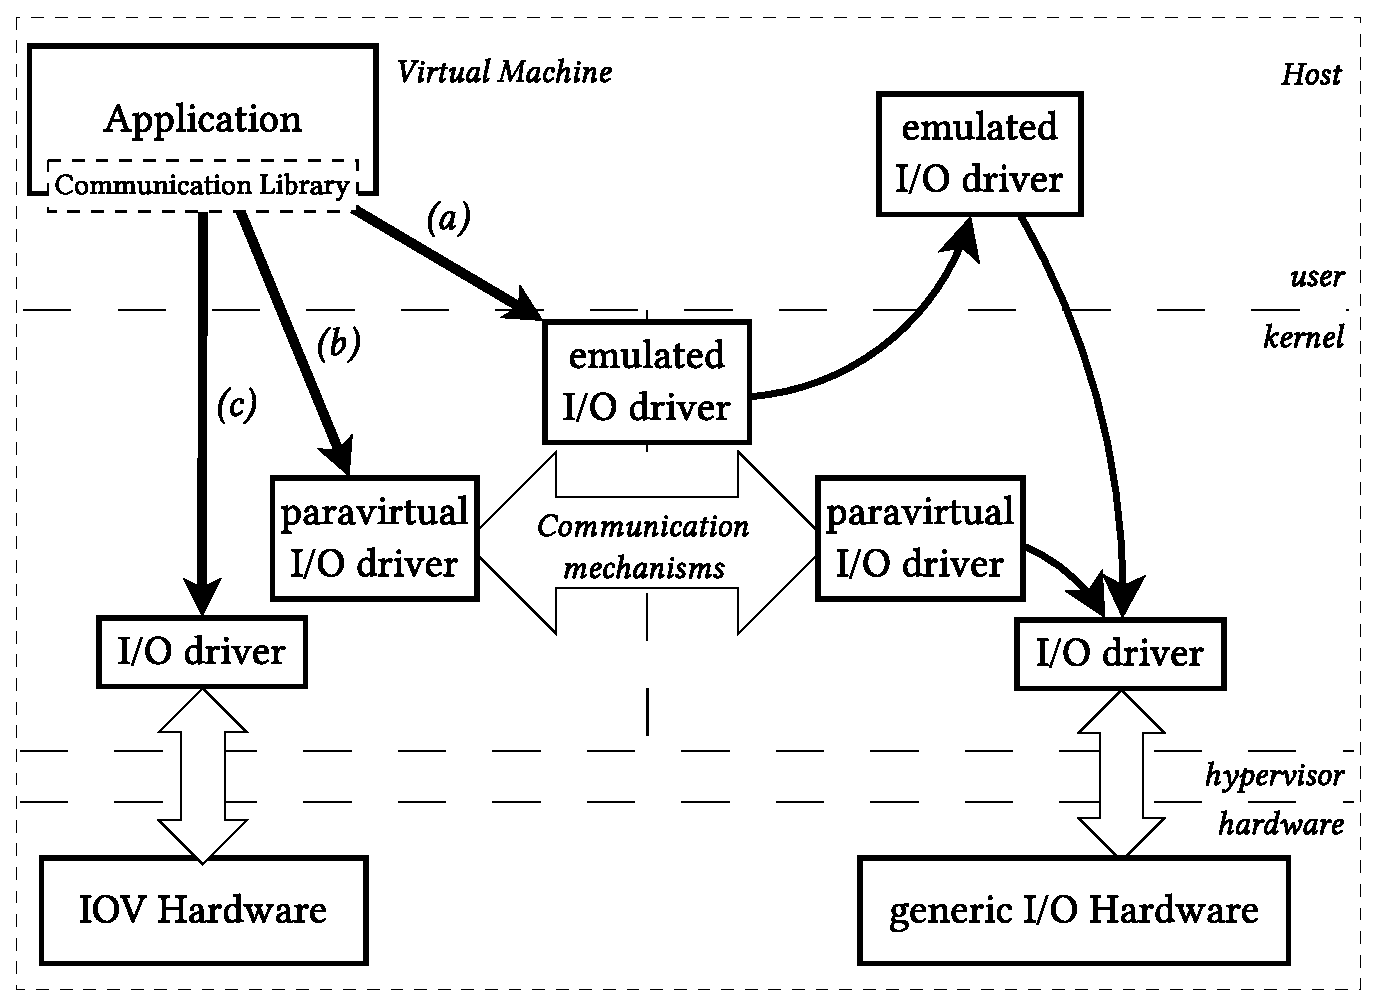
\includegraphics[width=\textwidth]{figs/bare/io_comm.eps}
\end{columns}
\end{frame}



\begin{frame}
\frametitle{I/O options in a Virtualized Environment: emulation}
\begin{columns}
\column{.8\textwidth}
\includegraphics[width=\textwidth]{figs/bare/io_emulated.eps}
%\note[item]{\tiny }
\end{columns}
\end{frame}

\begin{frame}
\frametitle{I/O options in a Virtualized Environment: paravirtual}
\begin{columns}
\column{.8\textwidth}
\includegraphics[width=\textwidth]{figs/bare/io_paravirt.eps}
\end{columns}
\end{frame}

\begin{frame}
\frametitle{I/O options in a Virtualized Environment: IOV}
\begin{columns}
\column{.8\textwidth}
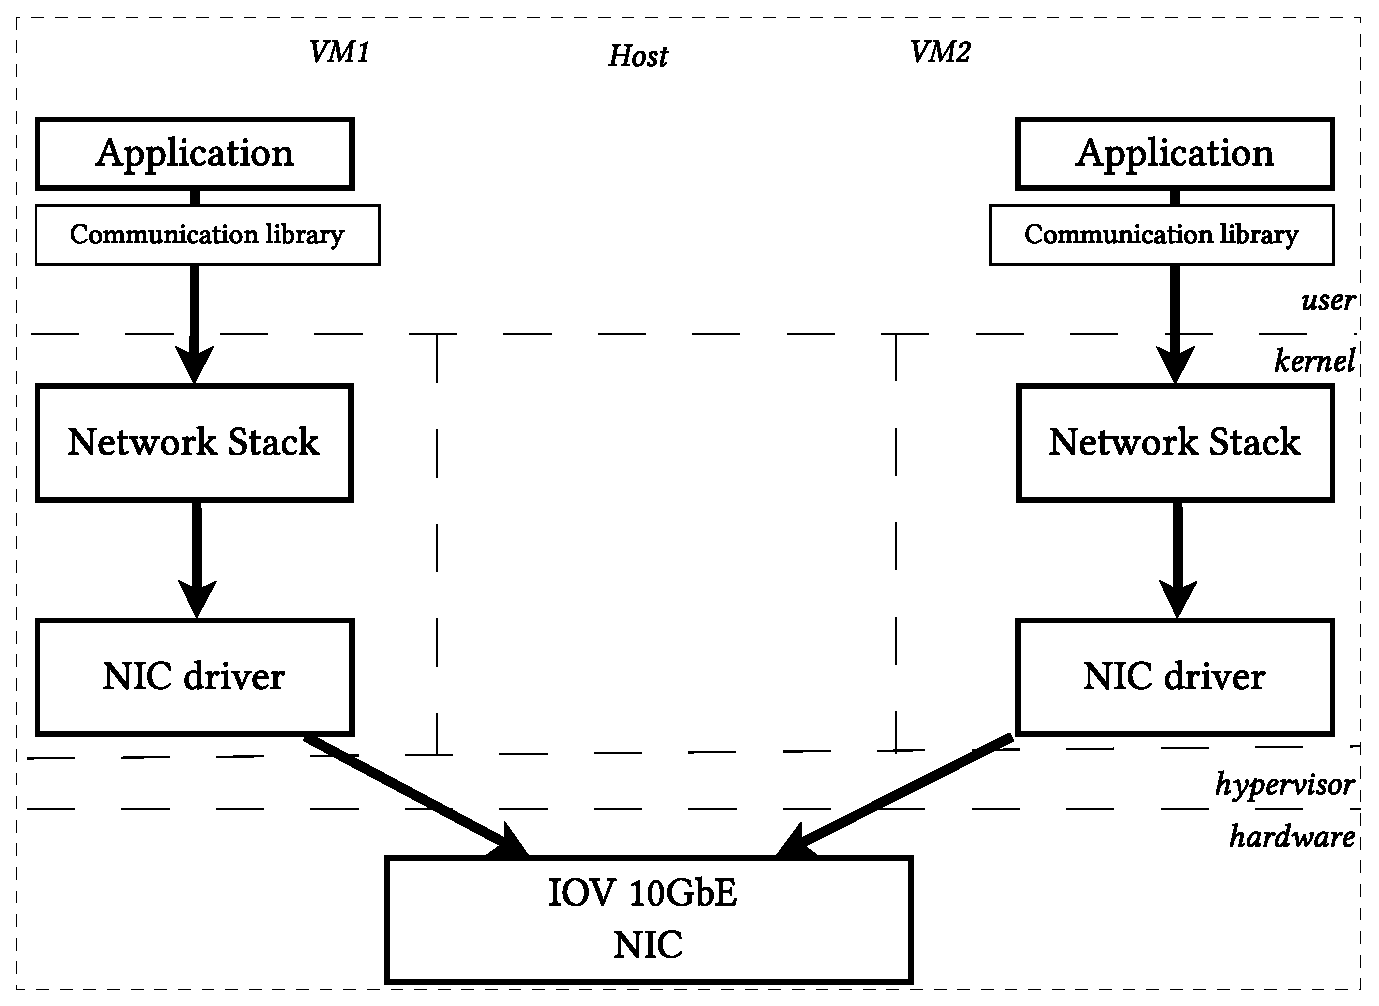
\includegraphics[width=\textwidth]{figs/bare/io_iov.eps}
\end{columns}
\end{frame}

\begin{frame}
\frametitle{I/O handling in popular open-source hypervisors}

\begin{block}{Parameters:}
\begin{itemize}
\item device emulation:
\begin{itemize}
\item totally unaware of the underlying platform -- fully flexible! (migration, checkpointing, etc.) (+)
%\pause
\item significant performance penatly (--)
\end{itemize}
\pause
\item paravirtual drivers
\begin{itemize}
\item needs extra effort to build the interface to the native driver (--)
\item scalable, as the interface to both VMs and the hardware is tailored to each driver class (+)
\end{itemize}
\pause
\item IOV: hardware multiplexing
\begin{itemize}
\item native drivers everywhere (+)
\item near-native performance (+)
\item intrusive in terms of hypervisor support (--)
\item inflexible (-)
\end{itemize}
\end{itemize}
\end{block}
%\pause
%\begin{columns}
%\centering
%\column{0.8\textwidth}
%\begin{block}{Proposal}
%Build a VM--aware interconnection framework to closely examine sources of overhead and set up
%efficient data paths
%\end{block}
%\end{columns}
\end{frame}

\begin{frame}
\begin{block}{I/O Virtualization (IOV)}
\begin{itemize}
\item direct data paths (near-native performance in terms of I/O)
\pause
\item flexibility, migration, scalability (?)
\end{itemize}
\end{block}

\pause
\begin{block}{}
In the era of multi/many--cores:
\begin{itemize}
\item VM containers will host a great number of VMs
\item are IOV adapters ready ?
\end{itemize}
\end{block}
\end{frame}

\subsection{Classes of I/O devices}

\begin{frame}
\frametitle{Characterizing I/O devices}
        \begin{block}{Block Devices}
		\begin{itemize} \item batching requests at block level --
                difficult to virtualize due to hardware characteristics (e.g. single set of
                spindles will serialize access -- needs a special interface to batch requests
                and then submit them)
                \end{itemize}
        \end{block}
        \begin{block}{Network devices}
                \begin{itemize}
                    \item batching transmision at packet level -- multiple queues (TX/RX)
                \end{itemize}
        \end{block}
        \begin{block}{Accelerator Hardware}
                \begin{itemize}
                    \item GPUs
                    \item FPGAs
                \end{itemize}
                both virtualizable depending on workload/hardware characteristics -- not yet implemented
        \end{block}
\end{frame}

\section{High-performance Interconnects}

\subsection{Basic Concepts}

\begin{frame}
\frametitle{High-performance Interconnects -- Basic concepts}
        \begin{block}{Endpoints}
                virtualized instance of a device -- logical source or destination of all communication
        \end{block}
        \begin{block}{Regions}
                sets of memory segments that contain virtually contiguous memory areas (allocated by the application)
        \end{block}
        \begin{block}{Events}
                \begin{itemize}
                \item user-level
                \item kernel-level
                \end{itemize}
                scalable method of communication between user--space and the hardware
        \end{block}
\end{frame}

\subsection{Native networking frameworks}
\begin{frame}
\frametitle{Open-MX software stack (user-level vs. traditional communication)}
\begin{columns}
\column{.8\textwidth}
\includegraphics[width=\textwidth]{figs/bare/open-mx-default.eps}
\end{columns}
\end{frame}

\subsection{Networking frameworks in VM environments}
\begin{frame}
\frametitle{Open-MX deployed in a bridged setup}
\begin{columns}
\column{.8\textwidth}
\includegraphics[width=\textwidth]{figs/bare/open-mx-xen.eps}
\end{columns}
\end{frame}
\begin{frame}

\frametitle{Open-MX deployed in an IOV setup}
\begin{columns}
\column{.8\textwidth}
\includegraphics[width=\textwidth]{figs/bare/open-mx-iov.eps}
\end{columns}
\end{frame}


\section{Xen2MX}

\subsection{Xen2MX Architecture}

\begin{frame}
\frametitle{Xen2MX architecture}
\begin{columns}
\column{.8\textwidth}
\includegraphics[width=\textwidth]{figs/bare/xen2mx.eps}
\end{columns}
\end{frame}

\begin{frame}
\frametitle{Xen2MX -- architecture details}
        \begin{block}{Frontend--Backend communication}
        \begin{itemize}
        \item consumer-producer scheme (soft-interrupts/polling)
        \item cyclic rings
        \item anticipatory handlers
        \end{itemize}
        \end{block}
        \begin{block}{Data Exchange (inter--/intra--node)}
        \begin{itemize}
        \item copies (\texttt{SMALL} messages)
        \item send \& receive queues (\texttt{MEDIUM} messages)
        \item regions (\texttt{LARGE} messages)
        \item grants (proactive):
                \begin{itemize}
                        \item pre-grant relevant memory space (both send and receive)
                        \item re-use grants
                \end{itemize}
        \end{itemize}
        \end{block}

\end{frame}


\begin{frame}
\frametitle{Xen2MX message exchange}
\begin{columns}
\column{.8\textwidth}
\includegraphics[width=\textwidth]{figs/bare/xen2mx_message_exchange.eps}
\end{columns}
\end{frame}


\begin{frame}
\frametitle{Xen2MX regions}
\begin{columns}
\column{.8\textwidth}
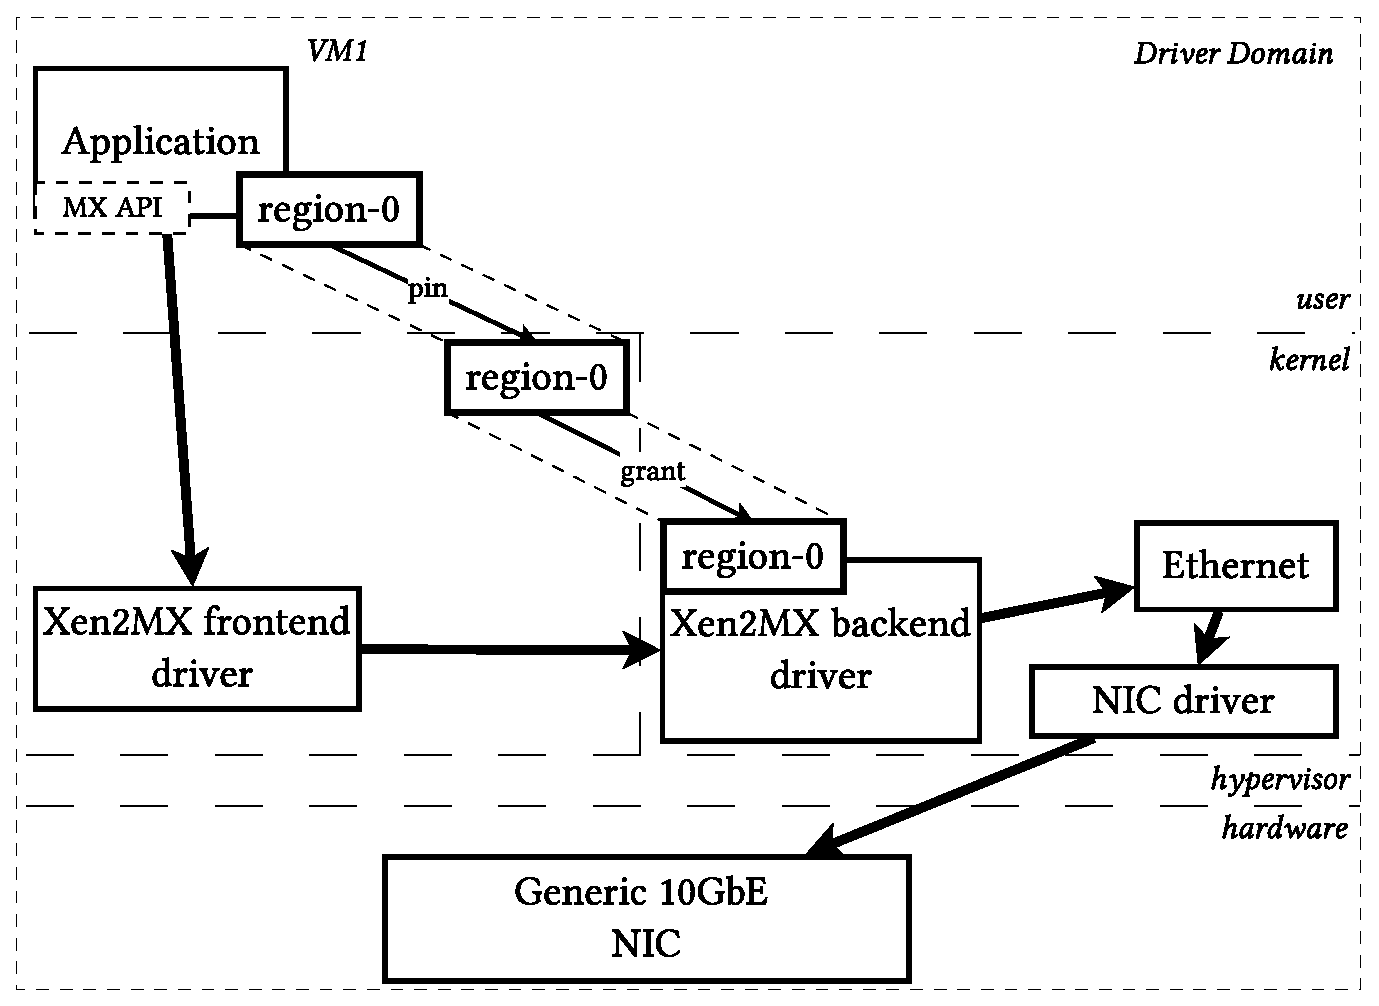
\includegraphics[width=\textwidth]{figs/bare/xen2mx_regions.eps}
\end{columns}
\end{frame}

\begin{frame}
\frametitle{Xen2MX API}
\begin{columns}
\column{.8\textwidth}
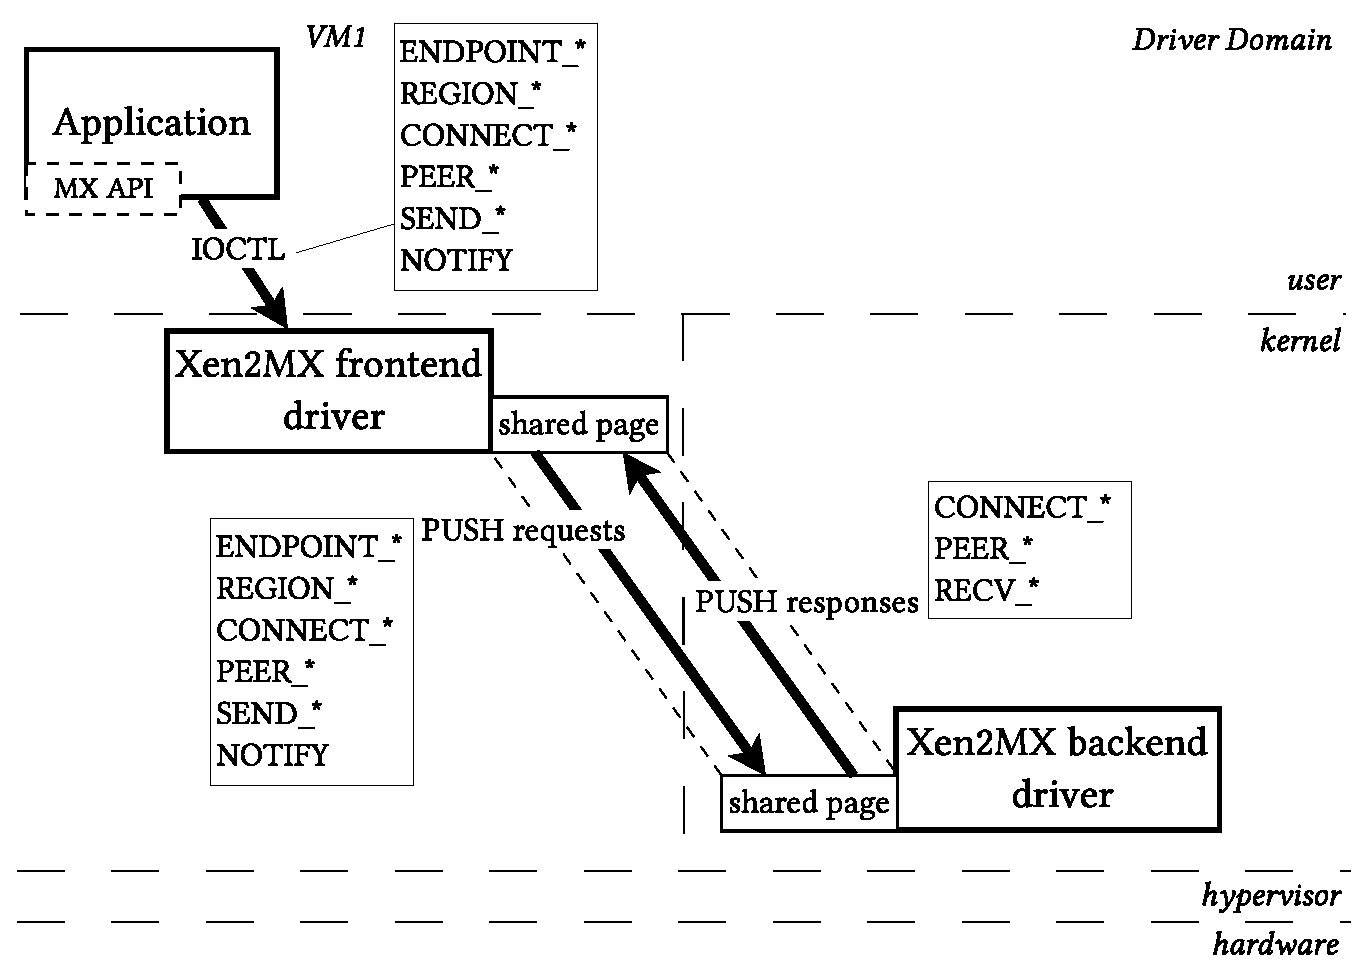
\includegraphics[width=\textwidth]{figs/bare/xen2mx_messages.eps}
\end{columns}
\end{frame}

\subsection{Xen2MX evaluation}

\begin{frame}
\frametitle{Xen2MX performance results}
\begin{block}{Testbed}
\begin{itemize}
\item 2x \{Intel Xeon @2.4Ghz, Intel 5500, 48GB memory, Generic 10GbE\}
\item Xen 4.2, Open-MX 1.5.2, Debian GNU/Linux (kernel version 3.4.0)
\item generic microbenchmark: \texttt{mx\_pingpong}
\begin{itemize}
%\item[\tiny{$\leq$ 64b}]: copying
%\item[\tiny{$\leq$ 32KB}]: send \& receive queues
%\item[\tiny{$\geq$ 64KB}]: rendez-vous semantics
\item$\leq$ 64b: copying
\item$\leq$ 32KB: send \& receive queues
\item$\geq$ 64KB: rendez-vous semantics
\end{itemize}
\end{itemize}
\end{block}
\begin{block}{Cases:}
\begin{itemize}
\item Native (no hypervisor)
\item PCI-attached (IOV-equivalent)
\item Bridged (Generic case)
\item Xen2MX (Plain, Tuned)
\end{itemize}
\end{block}
\end{frame}


\begin{frame}
\frametitle{Xen2MX performance results -- latency up to 16K }
\begin{columns}
\column{.8\textwidth}
\includegraphics[width=\textwidth]{figs/bare/latency_zoom.eps}
\end{columns}
\end{frame}

\begin{frame}
\frametitle{Xen2MX performance results -- latency}
\begin{columns}
\column{.8\textwidth}
\includegraphics[width=\textwidth]{figs/bare/lat_pingpong.eps}
\end{columns}
\end{frame}

\begin{frame}
\frametitle{Xen2MX performance results -- throughput}
\begin{columns}
\column{.8\textwidth}
\includegraphics[width=\textwidth]{figs/bare/bw_pingpong.eps}
\end{columns}
\end{frame}

\begin{frame}
\frametitle{Xen2MX performance results -- 512K messages}
\begin{columns}
\column{.8\textwidth}
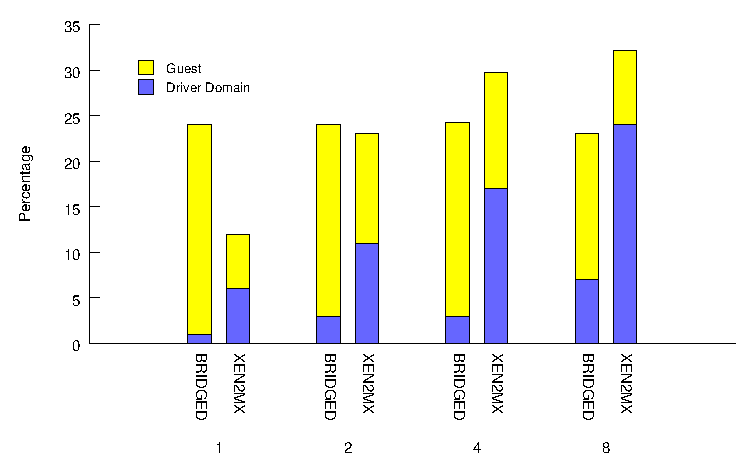
\includegraphics[width=\textwidth]{figs/bare/aggregate_doms_cpu.eps}
\end{columns}
\end{frame}

\begin{frame}
\frametitle{Xen2MX performance results -- 256K messages}
\begin{columns}
\column{.8\textwidth}
\includegraphics[width=\textwidth]{figs/bare/cpu_util.eps}
\end{columns}
\end{frame}

\begin{frame}
\frametitle{Xen2MX performance results -- scale up to 40 VMs}
\begin{columns}
\column{.8\textwidth}
\includegraphics[width=\textwidth]{figs/bare/scale_bw.eps}
\end{columns}
\end{frame}

\section{Conclusions}

\subsection{Summary}

\begin{frame}
\frametitle{Summary}
\begin{block}{I/O options in VM environments}
\begin{itemize}
\item emulated (when there is no other option)
\item split driver model (generic, scalable)
\item IOV (expensive but provides near-native performance)
\end{itemize}
\end{block}
\begin{block}{Xen2MX}
is a software port of the MX protocol to the Xen split driver model.
\end{block}
\begin{block}{Xen2MX benefits from:}
\begin{itemize}
\item all Open-MX features (MX binary compatibility, MXoE wire compatibility)
\item low-latency communication (almost as low as the IOV case)
\end{itemize}
\end{block}
%\begin{block}{Future Plans:}
%\begin{itemize}
%\item optimize Xen2MX to reach native performance numbers
%\item generalize the case to different hypervisors
%\end{itemize}
%\end{block}

Get Xen2MX!\\ \url{https://github.com/ananos/xen2mx}

\end{frame}

\begin{frame}
\frametitle
 %               \vfill%
%\begin{columns}
 %       \column{.75\textwidth}
                %\vfill%
            %    \begin{block}{}
                        {8th Workshop on Virtualization in High-performance Cloud Computing}
             %   \end{block}
                %\vfill%
                %\begin{block}{}
%\end{columns}
%\begin{itemize}
%\item Higher-level cloud architectures
%\item Lower-level design challenges for Hypervisors, VM-aware I/O devices
%\item Data Center management methods
%\item Nov 22nd, Denver, CO
\footnotesize 
%\begin{block}{Program}

\begin{tabular}{ll}
&
“The Benefits and Challenges of vHPC and Cloud Computing”\\
&Josh Simons, Office of the CTO, VMware\\
& “Integration of High-Performance Computing into a VCL Cloud”\\
&Patrick Dreher, MIT\\
&
"Archipelago: Unified Storage over Commodity Hardware using RADOS"\\
&Vangelis Koukis, Technical Lead, ~okeanos cloud at GRNET \\
%Coffee Break + Archipelago Demonstration  \\
&
“The Evolution of the ARM Architecture Towards Big Data and the Data-Centre”.\\
&John Goodacre, Director, Technology and Systems, ARM Processor Division \\
&
“Maximizing Performance with Cloud-Virtualized Dataflow Engine co-Processors”\\
&Jacob Bower, VP of Application Engineering, Maxeler Technologies. \\
&Closing Discussion 
\end{tabular}
%\end{block}

%\item Deadline: early july (provisional: July 1st)
%\end{itemize}

\begin{columns}
\column{.3\textwidth}
%        \begin{center}
                \includegraphics[scale=0.25]{figs/sighpc.eps}
                %\end{block}
                %\vfill%
%        \end{center}
\column{.3\textwidth}
 %       \begin{right}
                
\includegraphics[scale=0.26]{figs/SC13.eps}
 %       \end{right}
\end{columns}
\end{frame}

\begin{frame}
\frametitle{Thanks!}
                \vfill%
\begin{columns}
        \column{.35\textwidth}
        \begin{center}
                %\vfill%
            %    \begin{block}{}
        \begin{center}
                        {\LARGE Questions?}
        \end{center}
             %   \end{block}
                \vfill%
                %\vfill%
        \end{center}
\end{columns}
                \vfill%
\end{frame}

\begin{frame}
\frametitle{}
                \vfill%
\begin{columns}
        \column{.35\textwidth}
        \begin{center}
                %\vfill%
            %    \begin{block}{}
             %   \end{block}
                \vfill%
                %\vfill%
        \end{center}
\end{columns}
                \vfill%
\end{frame}

\begin{frame}
\frametitle{}
                \vfill%
\begin{columns}
        \column{.35\textwidth}
        \begin{center}
                %\vfill%
            %    \begin{block}{}
        \begin{center}
                        {\LARGE Backup}
        \end{center}
             %   \end{block}
                \vfill%
                %\vfill%
        \end{center}
\end{columns}
                \vfill%
\end{frame}

\begin{frame}
\frametitle{Xen2MX performance results -- Host CPU utilization}
\begin{columns}
\column{.8\textwidth}
\includegraphics[width=\textwidth]{figs/bare/lat_breakdown_dom0.eps}
\end{columns}
\end{frame}

\begin{frame}
\frametitle{Xen2MX performance results -- Guest CPU utilization}
\begin{columns}
\column{.8\textwidth}
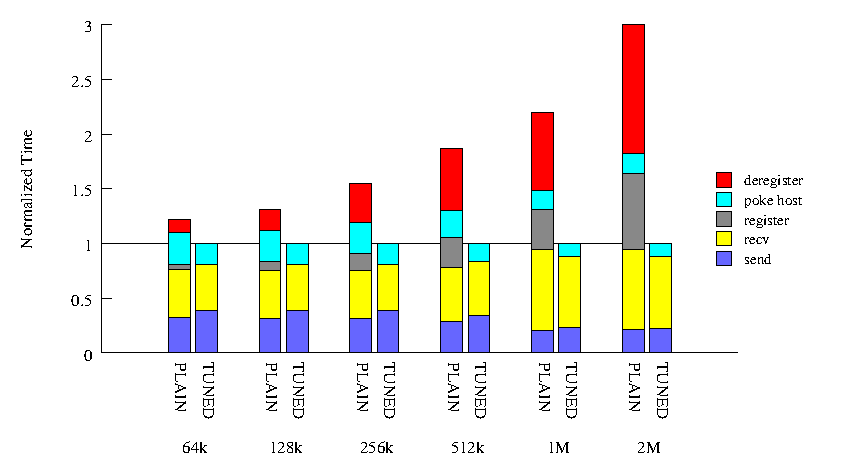
\includegraphics[width=\textwidth]{figs/bare/lat_breakdown_domU.eps}
\end{columns}
\end{frame}

\begin{frame}
\frametitle{Xen2MX steps -- I}
\begin{columns}
\column{.8\textwidth}
\includegraphics[width=\textwidth]{figs/bare/xen2mx_step1.pdf}
\end{columns}
\end{frame}

\begin{frame}
\frametitle{Xen2MX steps -- II}
\begin{columns}
\column{.8\textwidth}
\includegraphics[width=\textwidth]{figs/bare/xen2mx_step2.pdf}
\end{columns}
\end{frame}

\begin{frame}
\frametitle{Xen2MX steps -- III}
\begin{columns}
\column{.8\textwidth}
\includegraphics[width=\textwidth]{figs/bare/xen2mx_step3.pdf}
\end{columns}
\end{frame}

\begin{frame}
\frametitle{Xen2MX steps -- IV (Bridged)}
\begin{columns}
\column{.8\textwidth}
\includegraphics[width=\textwidth]{figs/bare/xen2mx_step4.pdf}
\end{columns}
\end{frame}

\begin{frame}
\frametitle{Xen2MX steps -- V (IOV)}
\begin{columns}
\column{.8\textwidth}
\includegraphics[width=\textwidth]{figs/bare/xen2mx_step5.pdf}
\end{columns}
\end{frame}

\begin{frame}
\frametitle{Xen2MX steps -- VI (Xen2MX)}
\begin{columns}
\column{.8\textwidth}
\includegraphics[width=\textwidth]{figs/bare/xen2mx_step6.pdf}
\end{columns}
\end{frame}

\end{document}
